\section{引言}

\begin{figure*}[t]
    \centering
    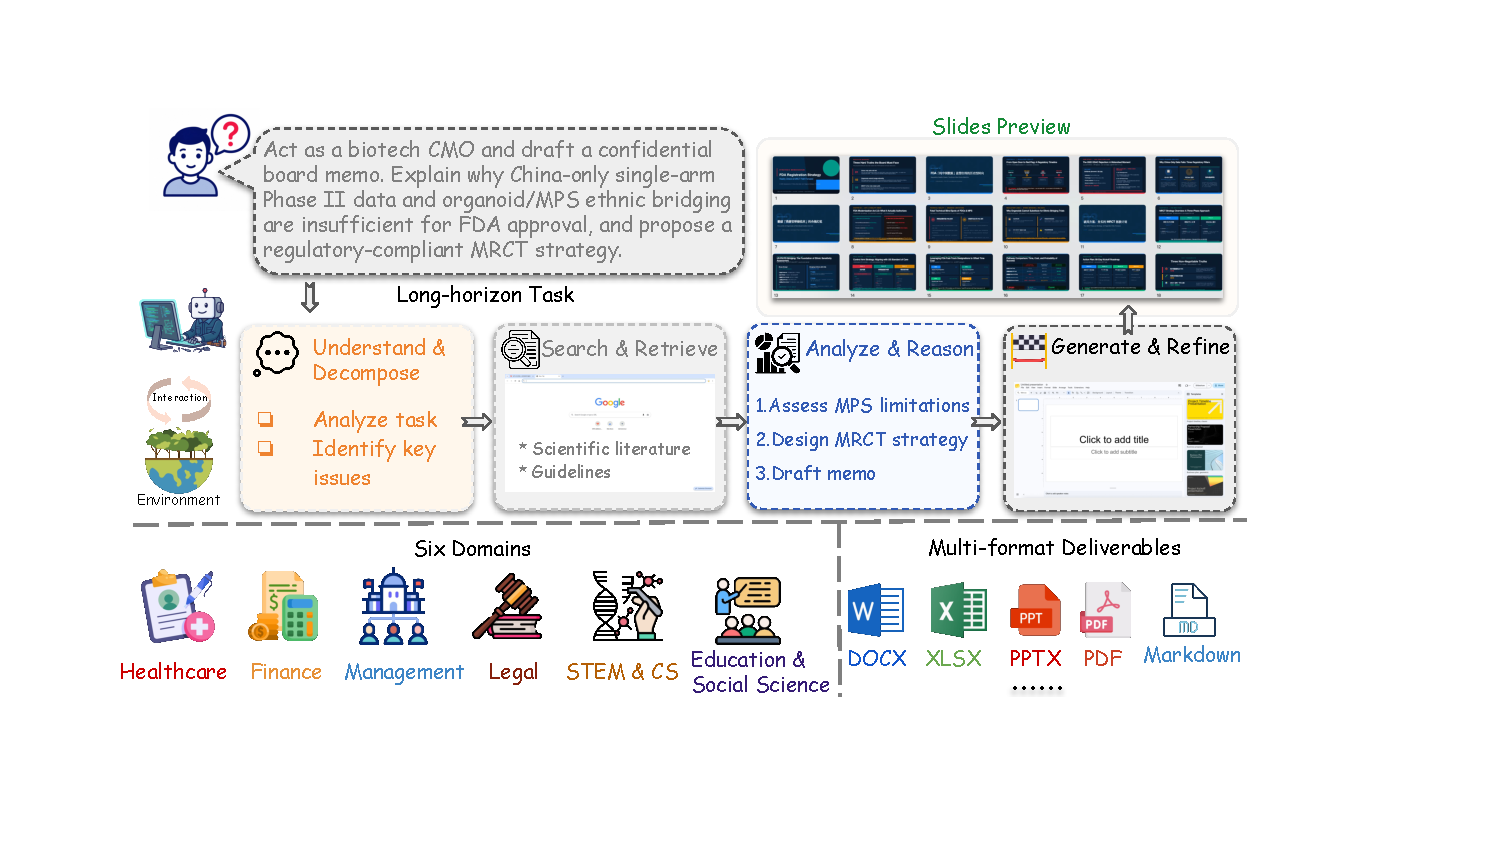
\includegraphics[width=0.9\textwidth]{figures/MainFig.pdf}
    \caption{StartupBench 概览：真实人工智能产品工作流、长时程智能体执行、六大领域覆盖以及多格式交付物生成。}
    \label{fig:bench_overview}
\end{figure*}

大语言模型（LLM）正日益从主要用于检索信息或回答问题的系统~\cite{du2026supergpqa,mialon2024gaia,wang2024mmlu}，演变为能够完成复杂现实任务的智能体。当前的人工智能系统被期望执行端到端（E2E）工作流、协调多种能力，并在现实约束下生成满足实际要求的交付物。随着人工智能不断融入专业工作，自主完成用户委派的任务已经成为衡量模型能力的重要标准。因此，评估人工智能系统能否可靠地把自身能力转化为可供专业使用的交付物，是下一代基准面临的一项核心挑战。

近期基准在现实环境下评估端到端任务执行方面取得了重要进展，但仍存在若干重要局限。第一，许多基准任务仍主要从研究者视角定义，而不是植根于已通过现实人工智能应用证明具有实际需求的工作流~\cite{phan2025humanity,patwardhan2025gdpval,mialon2024gaia}，因而难以反映真实的用户需求和交付物要求。第二，尽管一些基准会评估完整交付物~\cite{tang2026workspace,sun2026agents}，其评估协议往往远比交付物本身粗糙。现实工作成果通常涉及众多功能、结构、格式和领域特定要求，整体式评估无法如实检查这些要求。因此，现有基准对以下问题仍只能提供有限证据：\textit{当前模型和智能体在多大程度上能够满足复杂的现实用户要求，并可靠地产出可供专业使用的交付物？}

为解决这些局限，我们注意到，人工智能原生初创企业提供了一类天然的现实人工智能工作流来源：其产品已经过现实采用和商业需求验证，能够直接证明用户重视这些任务并希望将其委派给人工智能。因此，我们提出 \textbf{StartupBench}。这是一个由调研和访谈驱动的基准，它从这些工作流中提炼跨领域的现实端到端用户需求。StartupBench 涵盖 6 个主要领域的 97 项任务，并围绕以下设计原则构建：

\begin{itemize}
\item \textbf{以实际采用为基础的任务来源。}我们系统调研人工智能原生初创企业及其产品，并结合产品演示和用户访谈，识别已证明存在现实需求的工作流。随后，我们将这些工作流构造成基准任务，同时保留其核心用户目标和实际要求。

\item \textbf{端到端交付物。}每项任务都要求生成现实工作流中用户最终期望的完整交付物，而不是中间输出或简化演示。

\item \textbf{基于细粒度评分细则的评估。}每项 StartupBench 任务均使用多条相互独立的评分细则，覆盖预期交付物的不同维度，包括功能、结构、格式和领域特定质量，从而全面而如实地评估现实任务完成情况。
\end{itemize}

我们在统一智能体框架下使用 StartupBench 评估代表性模型。结果表明，即使最强模型也只能成功完成约 30\% 的基准任务，说明当前通用系统距离可靠生成可供专业使用的交付物仍相去甚远。不同领域之间的性能差异很大，其中金融、STEM 与计算机科学以及教育与人文学科尤其困难。进一步分析表明，这些失败主要源于复杂指令遵循和领域专门知识方面的局限，并据此指出未来基础模型和智能体系统值得推进的方向。

概括而言，我们的贡献如下：

\begin{itemize}
    \item 我们提出一种由调研和访谈驱动的方法，用于从真实人工智能采用场景构建智能体基准。
    \item 我们构建了 StartupBench。该基准经由人工智能原生初创企业调研、企业用户访谈、面向用户的任务抽象、专家数据构建和多阶段质量控制而形成。
    \item 我们针对当前基础模型和通用智能体在源自初创企业的工作流上的表现开展全面实证研究，为判断人工智能智能体是否正从“回答问题”迈向“可靠完成真实工作”提供实用评估信号。
\end{itemize}
